\section{Our Approach}

\begin{frame}
    \customframetitle{Our Approach}

    \centering

    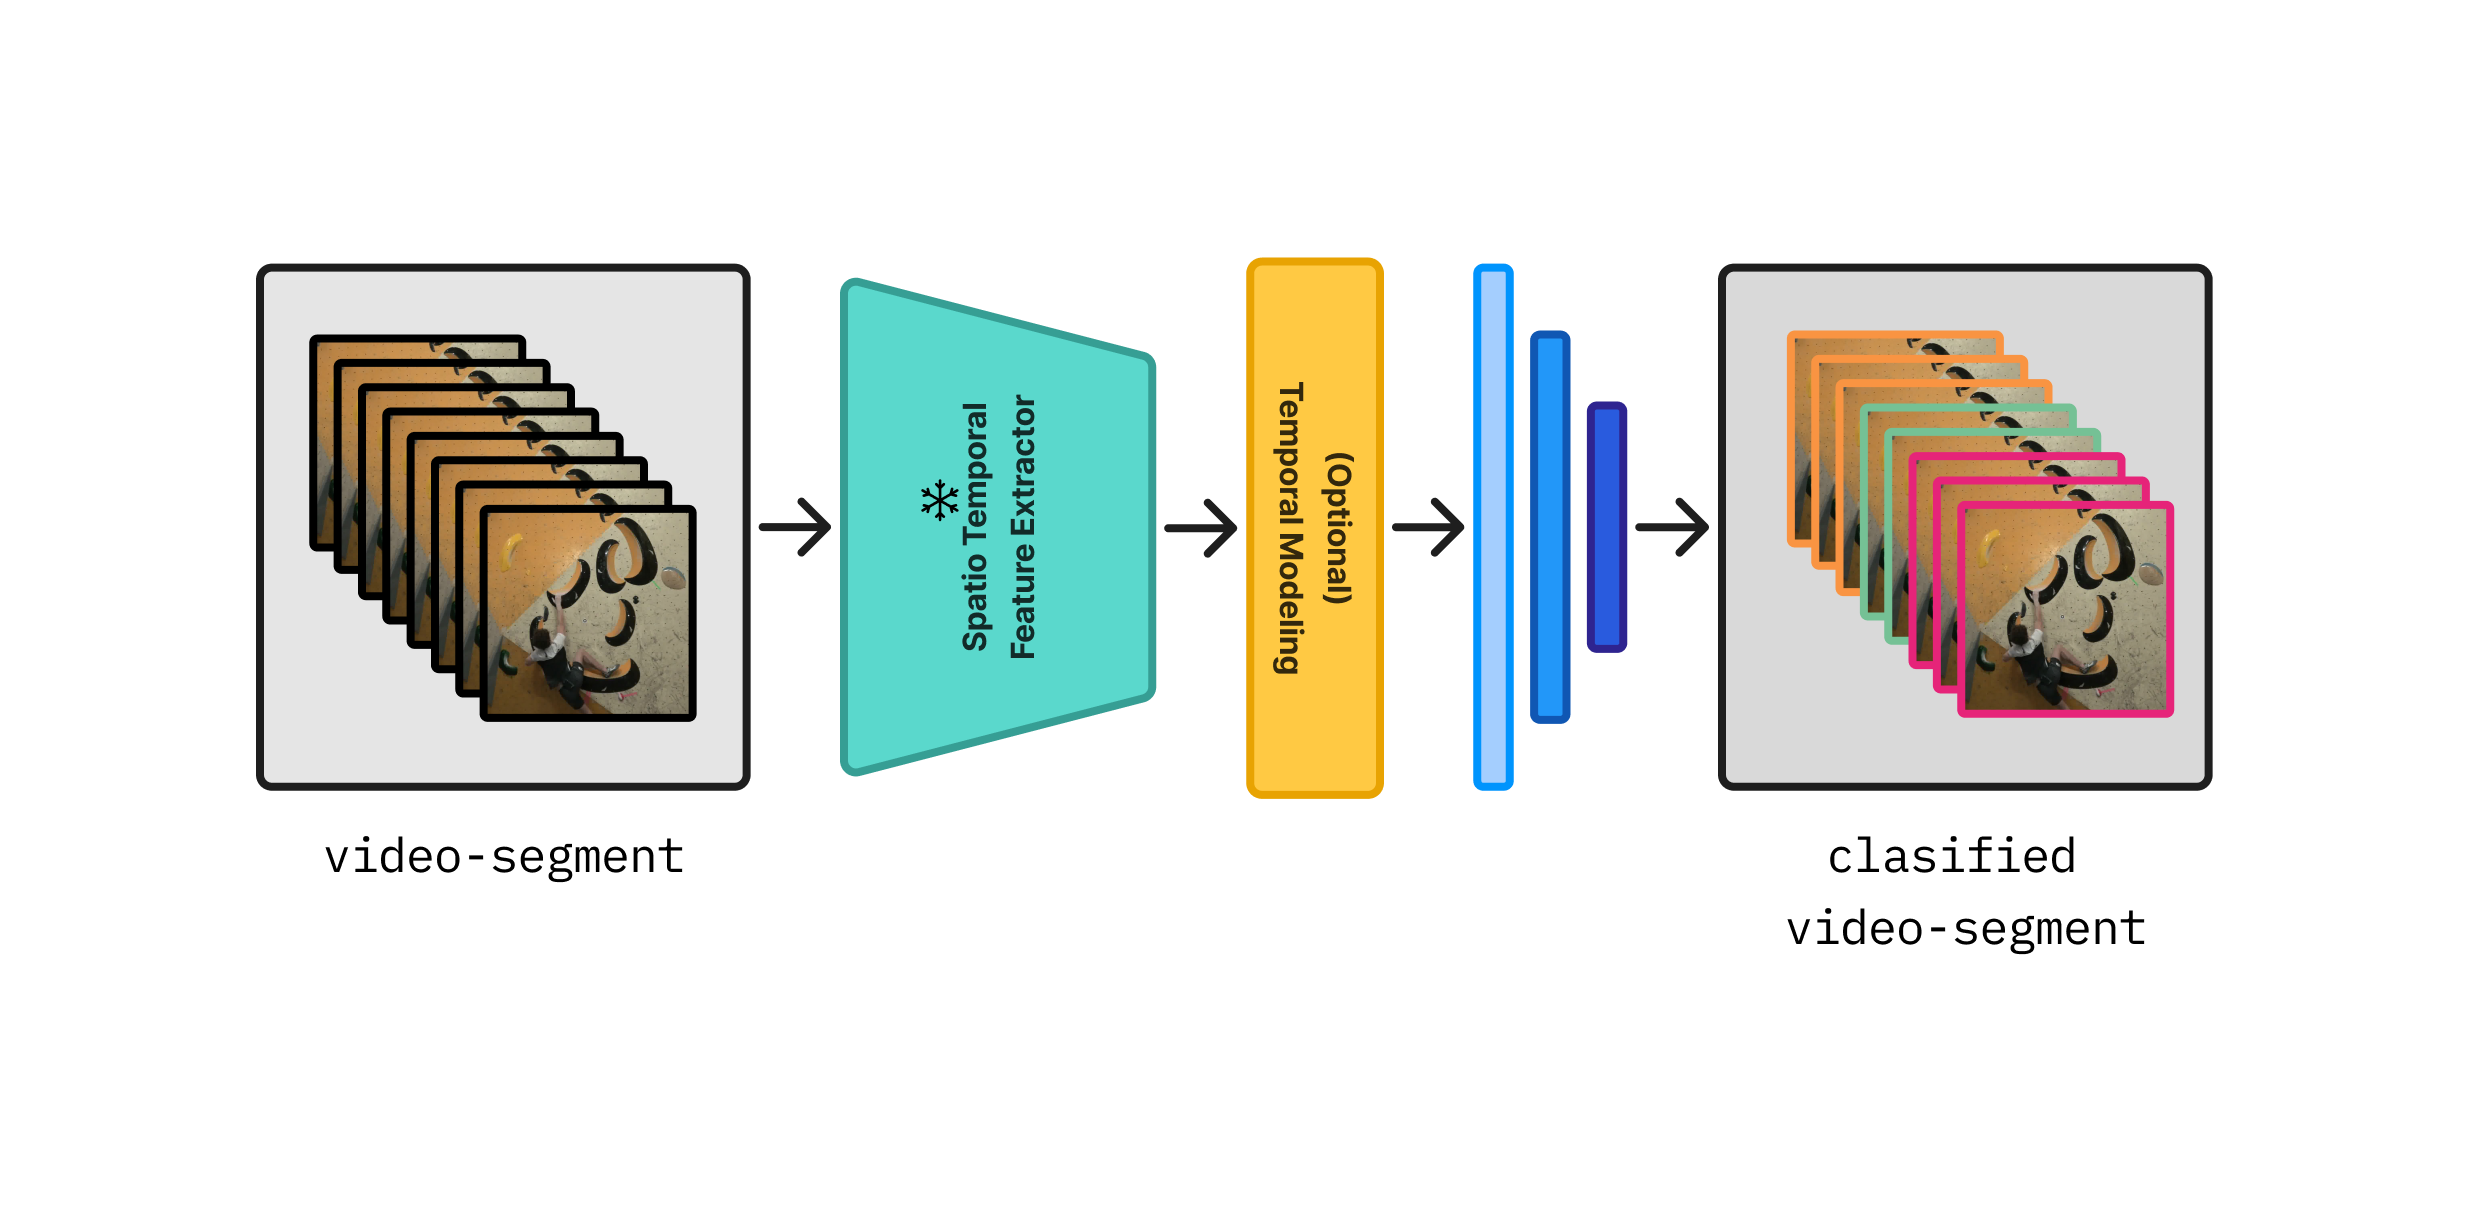
\includegraphics[width=1\textwidth]{../../assets/figures/model-overview.presentation.png}

    % TODO: do a similar figure: https://ai2-s2-public.s3.amazonaws.com/figures/2017-08-08/c1219c1334c292fb4e5fd0c434dacd0e1e4d5e28/2-Figure1-1.png
    % NOTE: big Schema to illustrate our approach.
\end{frame}

\begin{frame}
    \customframetitle{The Model's Input}

    \vspace{1em}

    \centering

    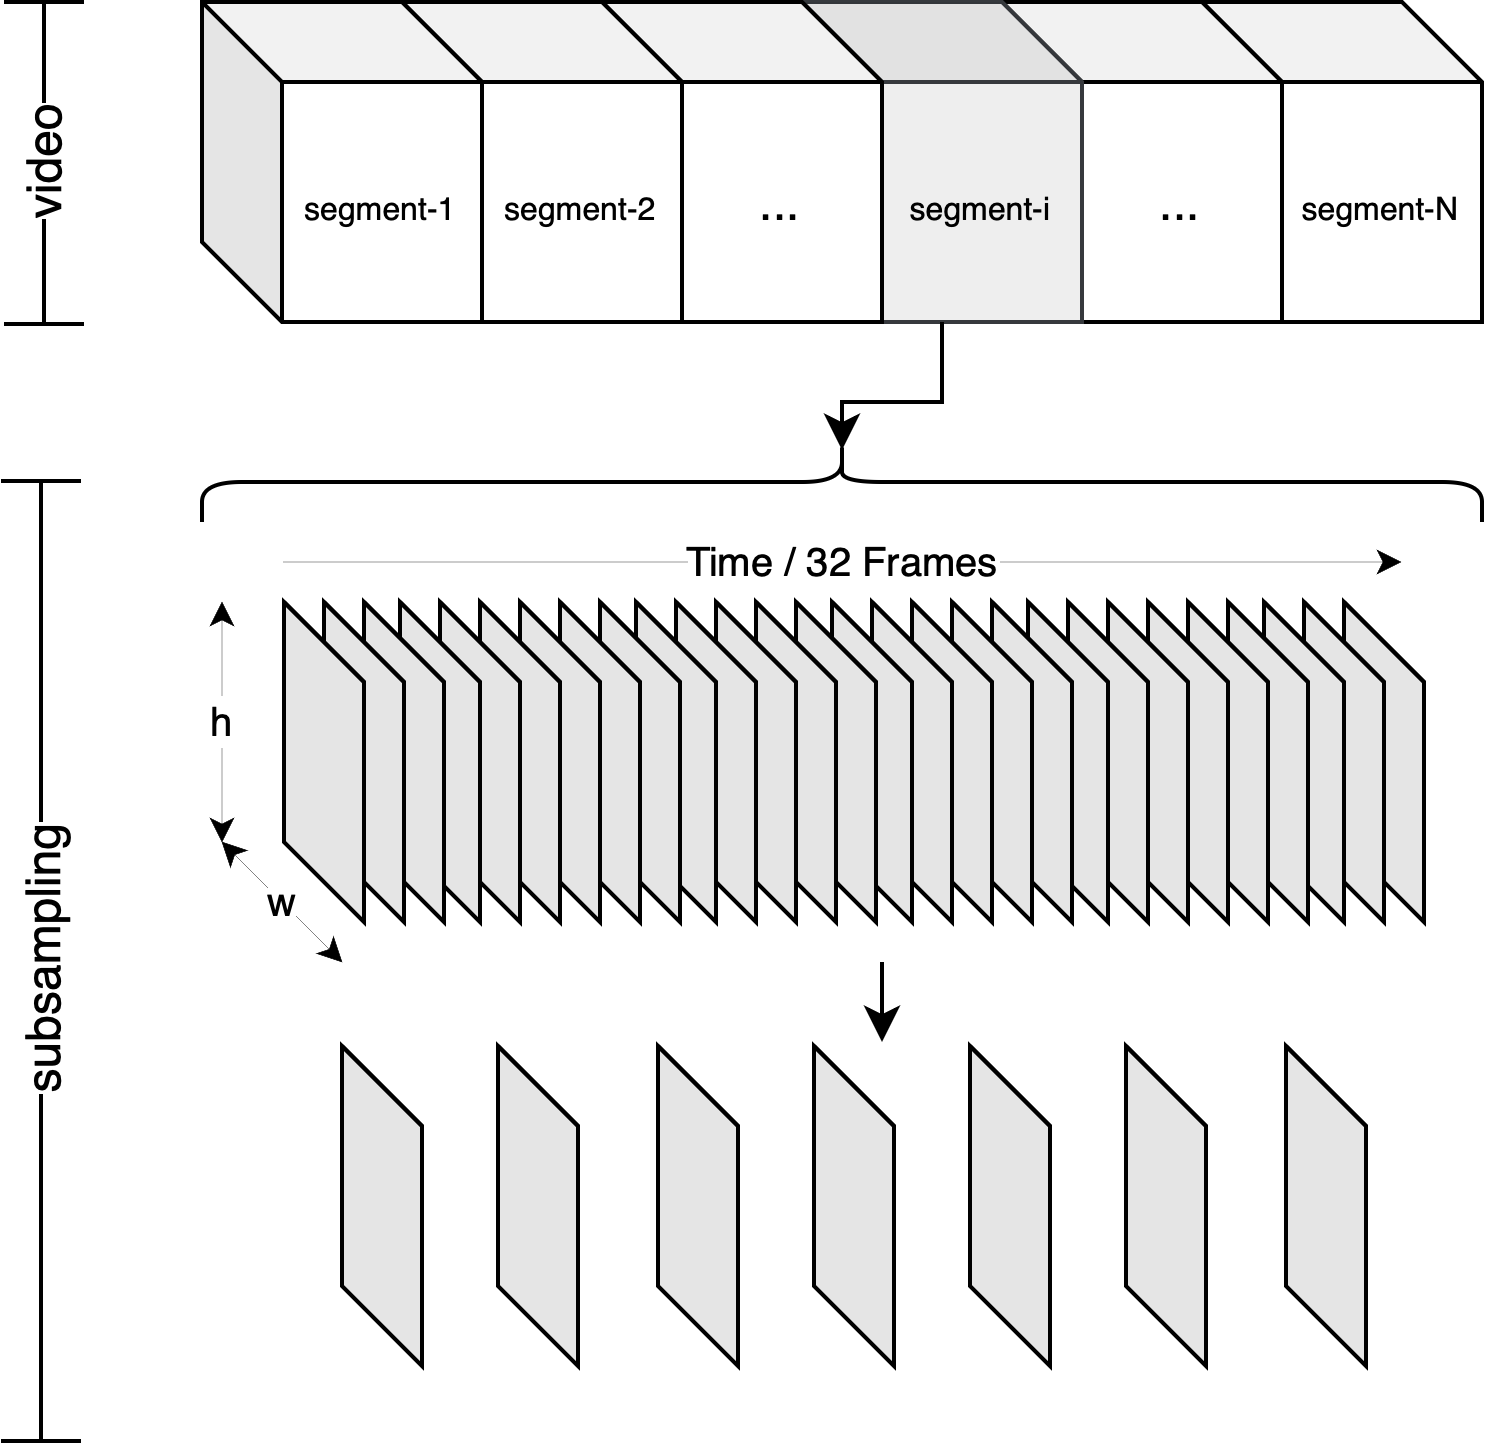
\includegraphics[width=0.45\textwidth]{../../assets/figures/subsampling.png}
\end{frame}

\begin{frame}
    \customframetitle{Spatio Temporal Feature Extractor}

    \begin{columns}
        \begin{column}{0.5\textwidth}
            \begin{figure}
                \centering
                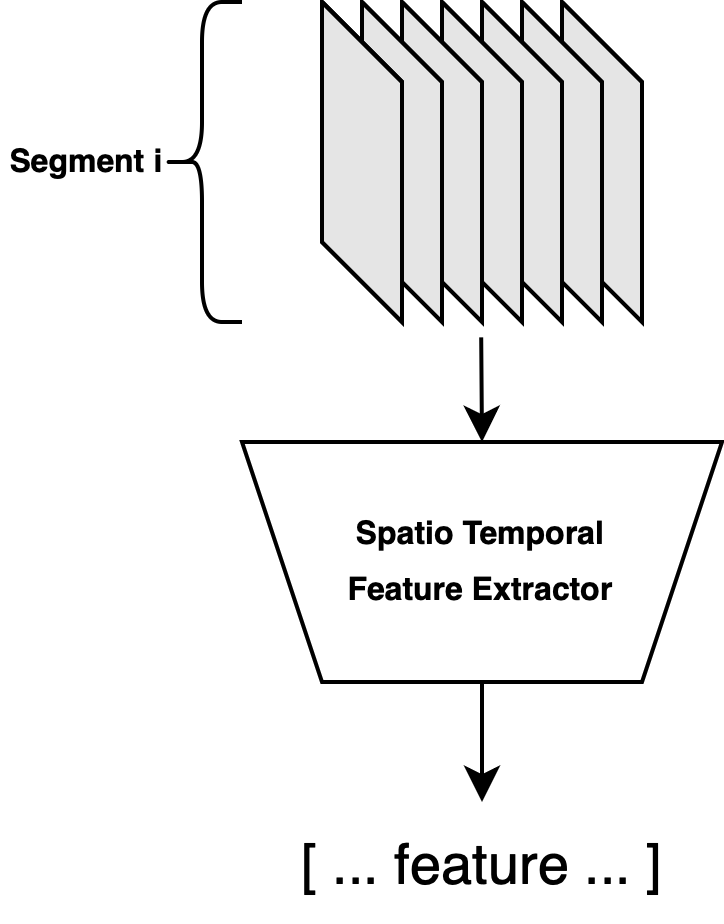
\includegraphics[width=0.65\linewidth]{../../assets/figures/segment-spatio-temporal-feature-extractor.png}
            \end{figure}
        \end{column}
        \begin{column}{0.5\textwidth}
            \begin{figure}
                \centering
                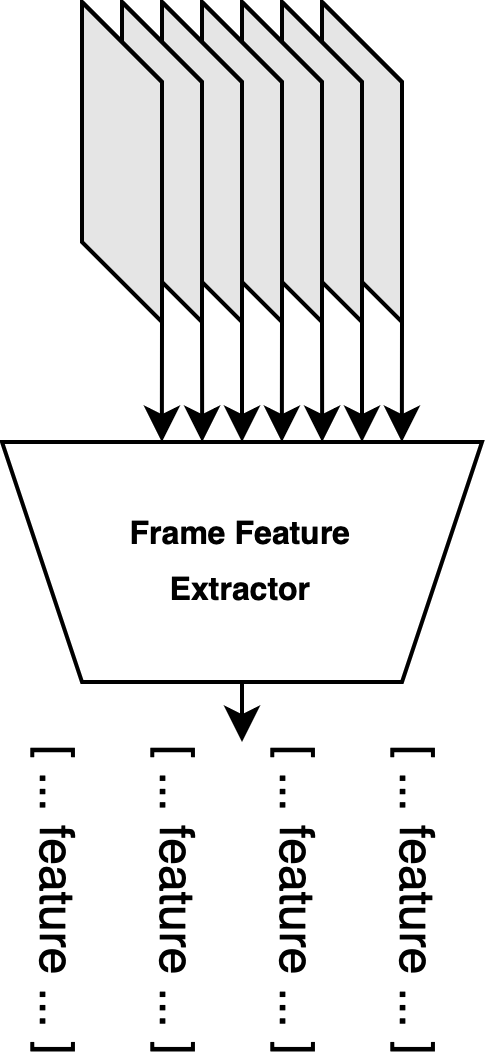
\includegraphics[width=0.40\linewidth]{../../assets/figures/frame-spatio-temporal-feature-extractor.png}
            \end{figure}
        \end{column}
    \end{columns}
\end{frame}

\begin{frame}
    \customframetitle{Features Aggregation}

    \vspace{1em}

    This step is necessary for Frame based feature extractors.

    \vspace{1em}

    \begin{itemize}
        \itemsep1em
        \item \textbf{Concatenation}.
        \item Averaging.
        \item LSTM Modeling.
        \item Summation.
    \end{itemize}
\end{frame}

\begin{frame}
    \customframetitle{Examples of Spatio Temporal Feature Extractors}

    \vspace{1em}

    \begin{figure}
        \centering
        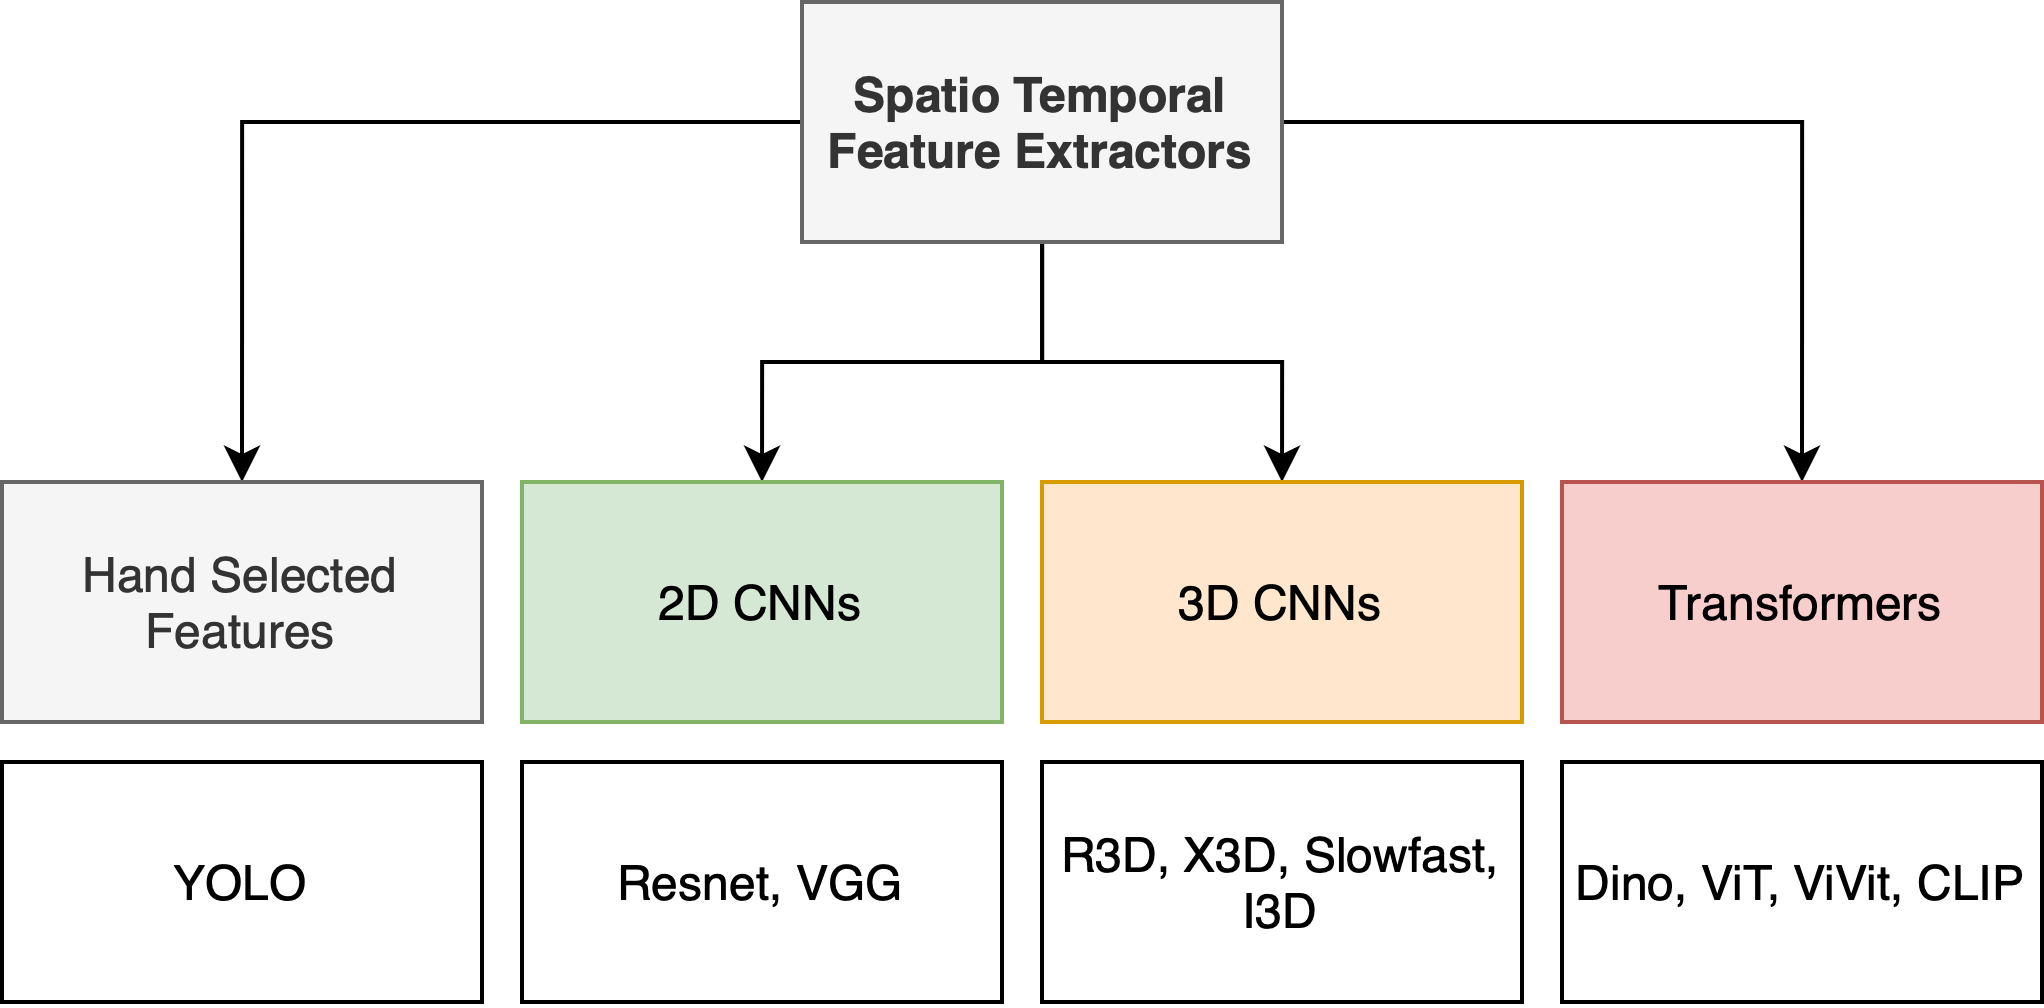
\includegraphics[width=0.85\linewidth]{../../assets/figures/examples-of-spatio-temporal-feature-extractors.png}
    \end{figure}

\end{frame}

\begin{frame}
    \customframetitle{Classifier}

    \vspace{1em}

    \centering

    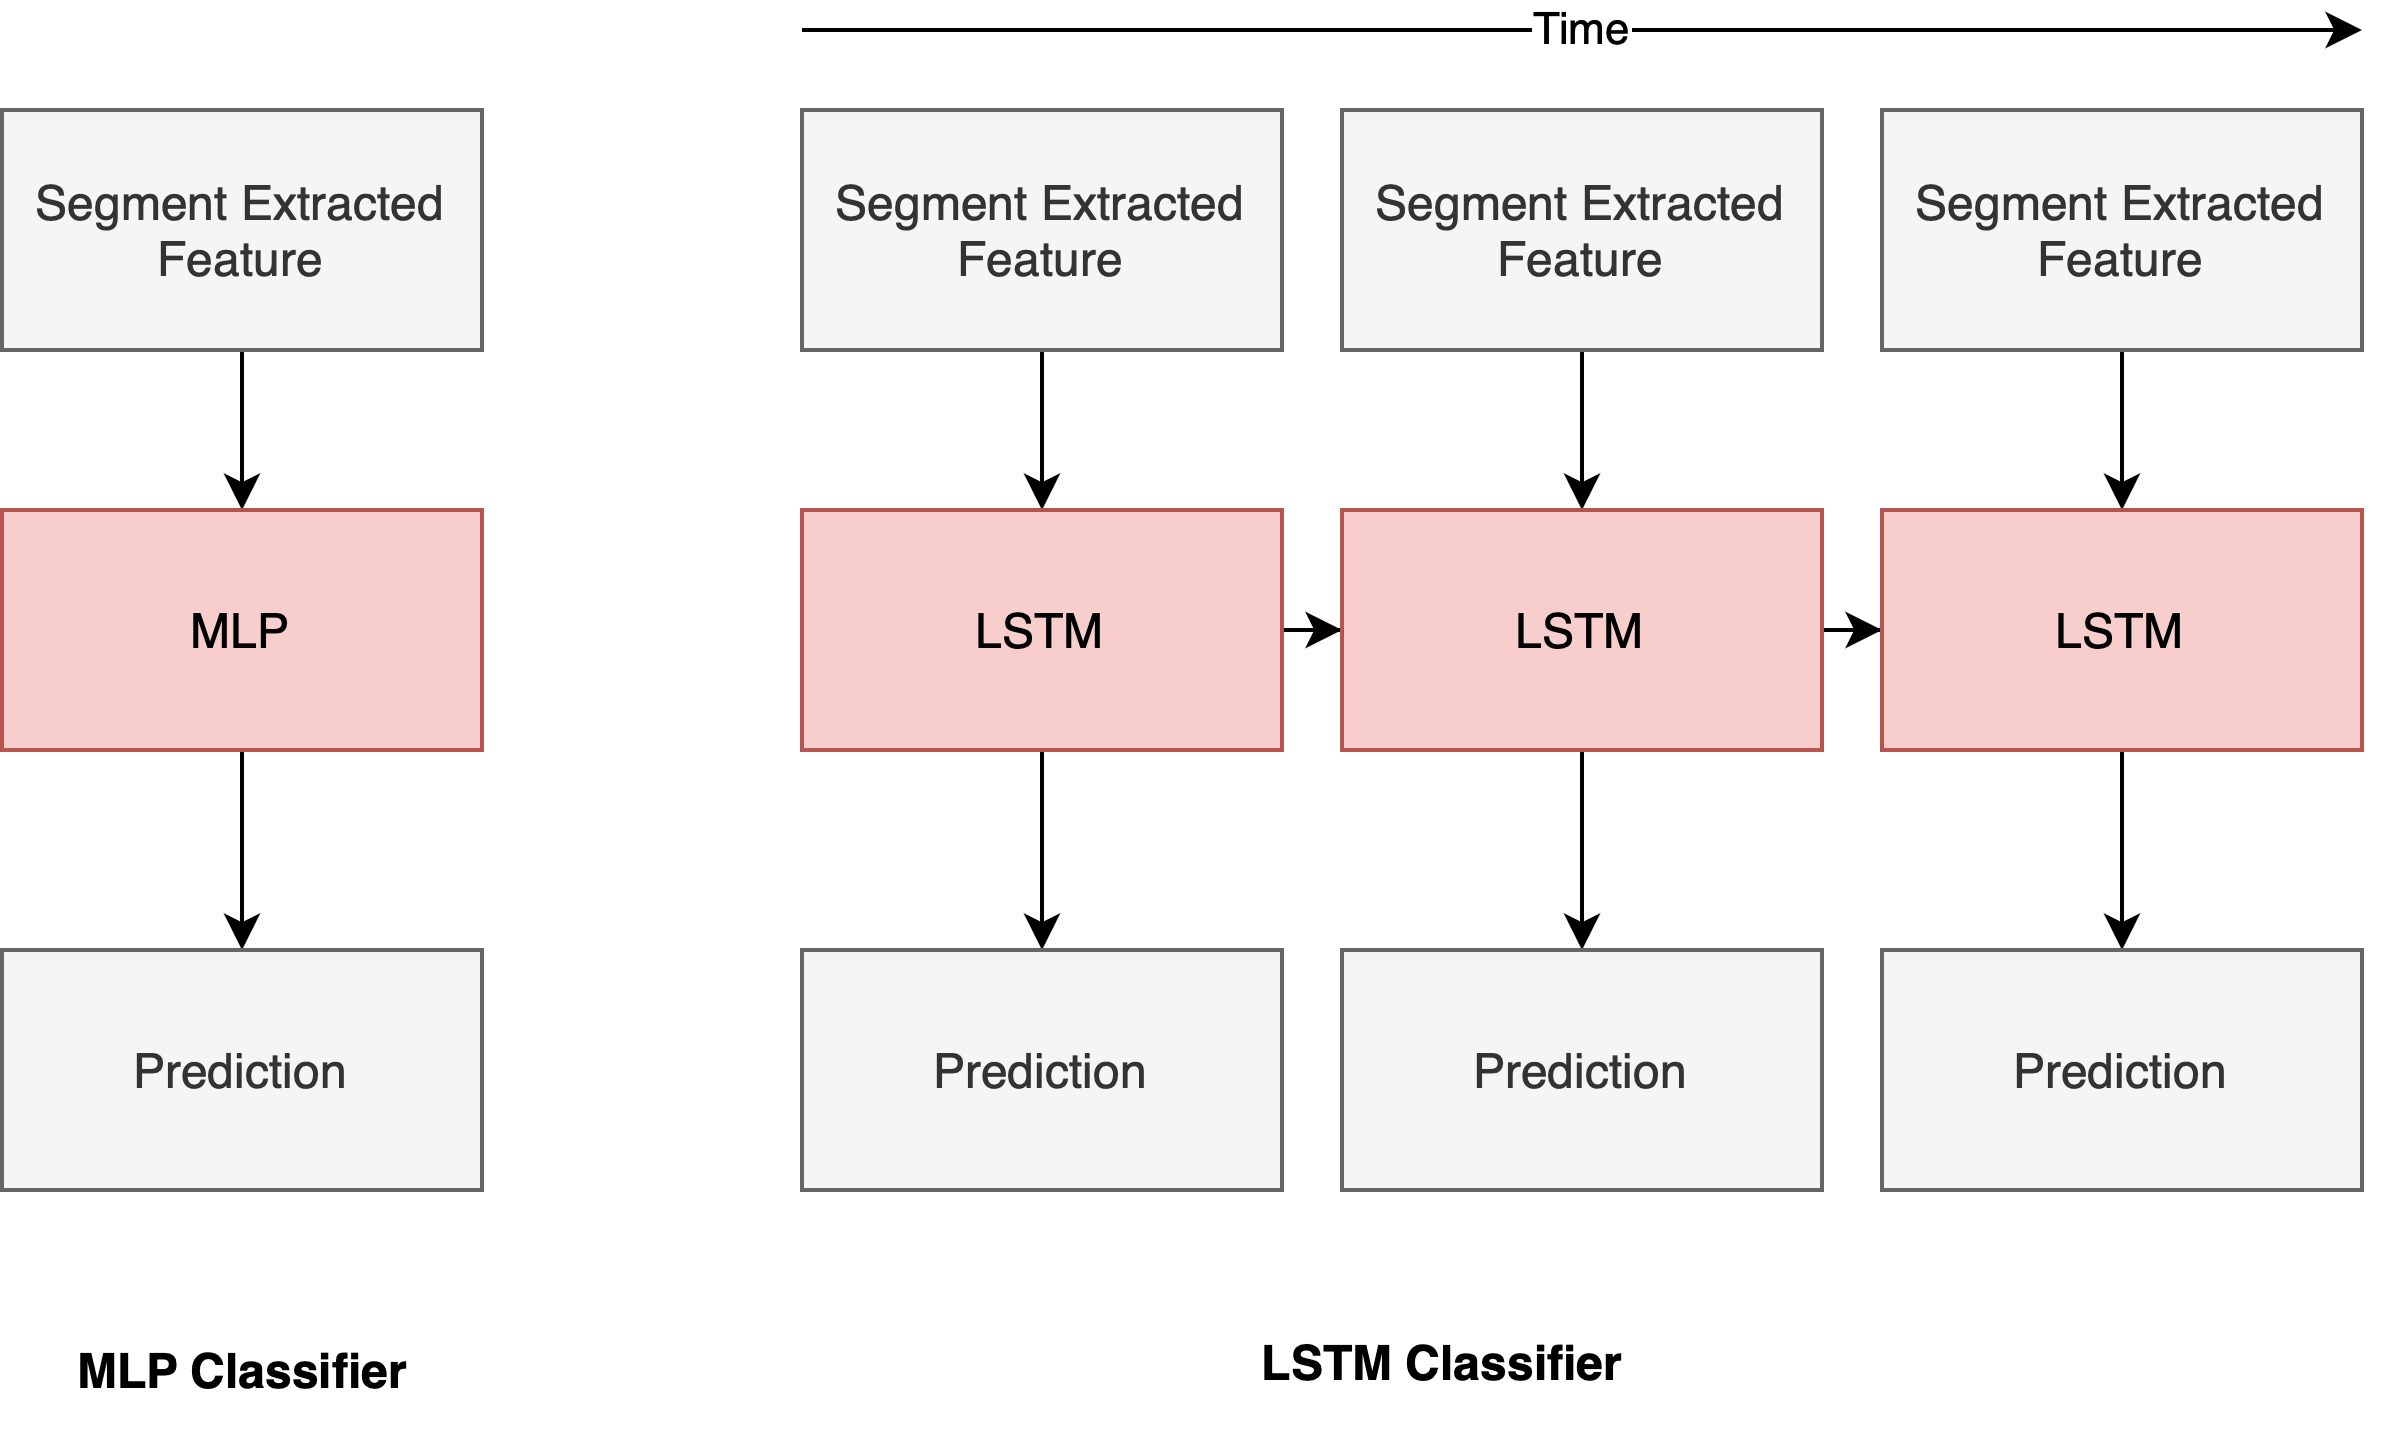
\includegraphics[width=0.75\textwidth]{../../assets/figures/classifier.presentation.png}
\end{frame}

\begin{frame}
    \customframetitle{Training Setup}

    \vspace{1em}

    \begin{itemize}
        \itemsep1em
        \item Used cross-entropy loss, with potential to explore focal or label-smoothing loss.
        \item Prevented data leakage by keeping segments from the same video in the same set.
        \item Removal of personless frames, cleaning data, and removing stopwatch segments.
        \item Developed a custom Python package (cached-dataset) for faster data loading.
        \item Combined pre-trained models, temporal sub-sampling, and filtering for efficient training.
    \end{itemize}
\end{frame}

% NOTE: state that the approach is fully parallelizable.